\section{Roles of Network Components}
\label{sec:components}

There are $6$ physical components in our network in total, of which $3$ are Cisco routers and the other $3$ are TOSHIBA laptops. Each component plays an important role in the network as shown in Figure \ref{fig:roles}.

\begin{figure}[t!]
    \centering
    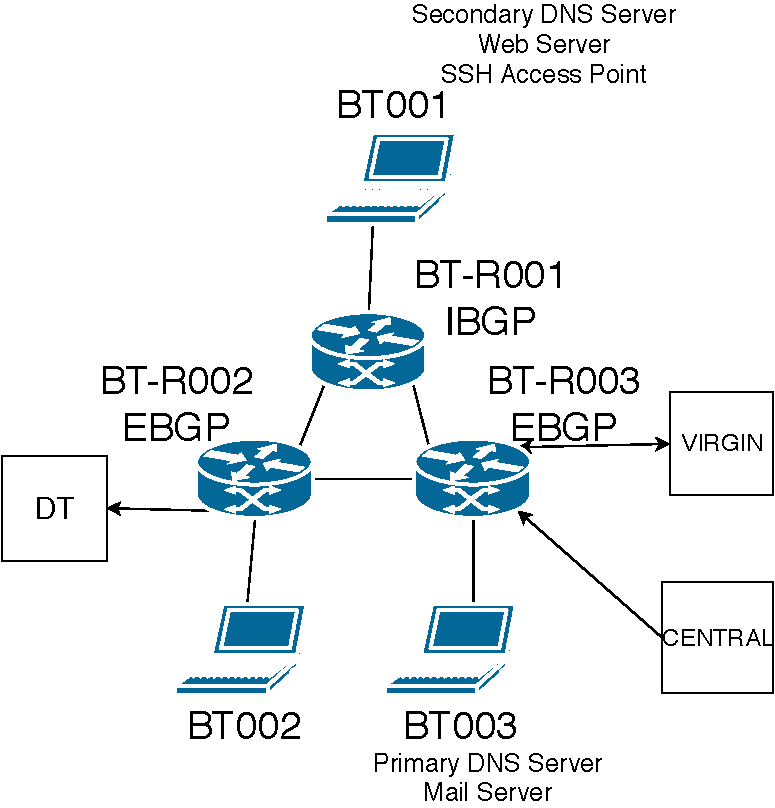
\includegraphics[width=\linewidth]{roles}
    \caption{Roles of Main Components in BT Network.}
    \label{fig:roles}
\end{figure}

\subsection{Routers}
In terms of connection, each router is attached with one customer subnet and thus providing Internet service to one customer. Router 1 (BT-R001) is not physically conncted to any outside network. Router 2 (BT-R002) is connected to DT Network and Router 3 (BT-R003) is connected to Virgin Network and Central Network through cables.

In terms of routing, all routers are Level-1 routers in intra-domain IS-IS routing protocol. In BGP routing protocol, Router 1 (BT-R001) acts as an Internal BGP (IBGP) router while Router 2 (BT-R002) and Router 3 (BT-R003) act as External BGP (EBGP) routers. 



\subsection{Laptops}

All laptops are running a Ubuntu 16.04 system. Each of them is connected to a customer subnet thourgh a cable. 
In terms of services, Laptop 1 (BT001) provides DNS service for \texttt{bt.lboro} as a secondary DNS server and WWW service at \texttt{http://bt.lboro}. It also acts as a secure SSH access point to routers for administrative purposes. 
Laptop 2 (BT002) doesn't provide any service and thus acts act an normal user in the network. 
Laptop 3 (BT003) provides DNS service for \texttt{bt.lboro} as a primary DNS server. In addition, it hosts Email service at \texttt{bt.lboro}.

